\documentclass{standalone}
\usepackage{tikz}
\usetikzlibrary{patterns, positioning}
\usepackage[sfdefault]{ClearSans} %% option 'sfdefault' activates Clear Sans as the default text font
\usepackage[T1]{fontenc}

\begin{document}
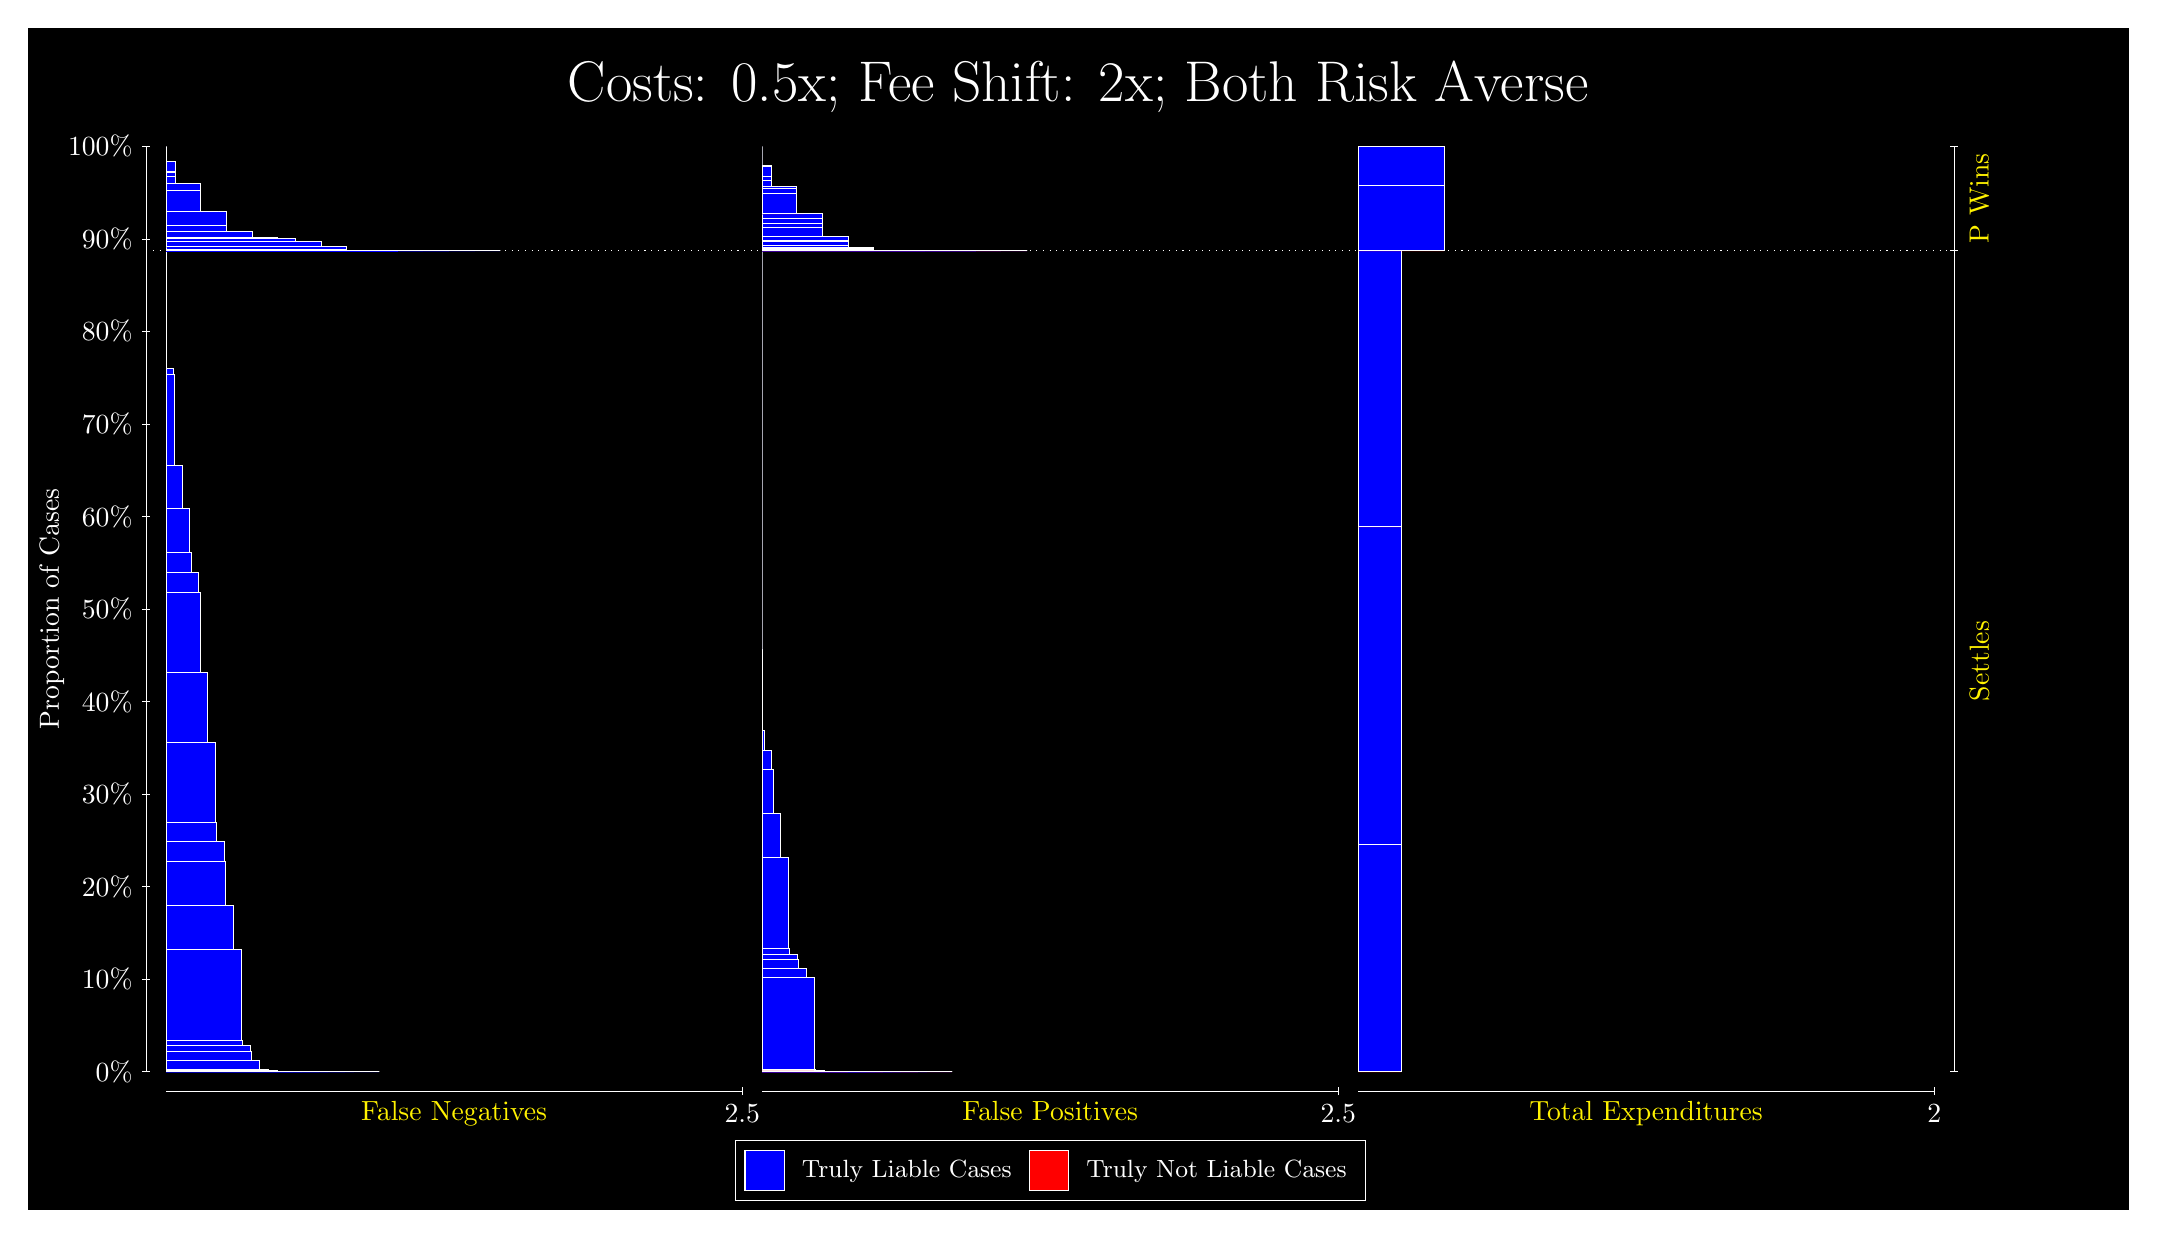
\begin{tikzpicture}
\draw[fill=black] (0,0) rectangle (26.667,15);
\draw[text=white] (0,13.5) rectangle (26.667,15) node[midway] {\huge Costs: 0.5x; Fee Shift: 2x; Both Risk Averse};
\draw[white, very thin] (1.5,1.75) -- (1.5,13.5);
\node[rotate=90, text=white, anchor=center] at (0.3, 7.625) {Proportion of Cases};
\draw[white, very thin] (1.45,1.75) -- (1.55,1.75);
\node[text=white, anchor=east] at (1.45, 1.75) {0\%};
\draw[white, very thin] (1.45,2.925) -- (1.55,2.925);
\node[text=white, anchor=east] at (1.45, 2.925) {10\%};
\draw[white, very thin] (1.45,4.1) -- (1.55,4.1);
\node[text=white, anchor=east] at (1.45, 4.1) {20\%};
\draw[white, very thin] (1.45,5.275) -- (1.55,5.275);
\node[text=white, anchor=east] at (1.45, 5.275) {30\%};
\draw[white, very thin] (1.45,6.45) -- (1.55,6.45);
\node[text=white, anchor=east] at (1.45, 6.45) {40\%};
\draw[white, very thin] (1.45,7.625) -- (1.55,7.625);
\node[text=white, anchor=east] at (1.45, 7.625) {50\%};
\draw[white, very thin] (1.45,8.8) -- (1.55,8.8);
\node[text=white, anchor=east] at (1.45, 8.8) {60\%};
\draw[white, very thin] (1.45,9.975) -- (1.55,9.975);
\node[text=white, anchor=east] at (1.45, 9.975) {70\%};
\draw[white, very thin] (1.45,11.15) -- (1.55,11.15);
\node[text=white, anchor=east] at (1.45, 11.15) {80\%};
\draw[white, very thin] (1.45,12.325) -- (1.55,12.325);
\node[text=white, anchor=east] at (1.45, 12.325) {90\%};
\draw[white, very thin] (1.45,13.5) -- (1.55,13.5);
\node[text=white, anchor=east] at (1.45, 13.5) {100\%};

\draw[white, very thin] (24.457,1.75) -- (24.457,13.5);
\draw[white, very thin] (24.407,1.75) -- (24.507,1.75);
\node[anchor=west] at (24.407, 1.75) {};
\draw[white, very thin] (24.407,12.175) -- (24.507,12.175);
\node[anchor=west] at (24.407, 12.175) {};
\draw[white, very thin] (24.407,13.5) -- (24.507,13.5);
\node[anchor=west] at (24.407, 13.5) {};

\draw[white, very thin, fill=blue] (1.75,1.75) rectangle (4.458,1.75);
\draw[white, very thin, fill=blue] (1.75,1.75) rectangle (4.1327,1.75);
\draw[white, very thin, fill=blue] (1.75,1.75) rectangle (4.0188,1.75);
\draw[white, very thin, fill=blue] (1.75,1.75) rectangle (3.8074,1.75);
\draw[white, very thin, fill=blue] (1.75,1.75) rectangle (3.6936,1.75);
\draw[white, very thin, fill=blue] (1.75,1.75) rectangle (3.5797,1.7501);
\draw[white, very thin, fill=blue] (1.75,1.7501) rectangle (3.4821,1.7501);
\draw[white, very thin, fill=blue] (1.75,1.7501) rectangle (3.3683,1.7502);
\draw[white, very thin, fill=blue] (1.75,1.7502) rectangle (3.2544,1.7563);
\draw[white, very thin, fill=blue] (1.75,1.7563) rectangle (3.1568,1.7615);
\draw[white, very thin, fill=blue] (1.75,1.7615) rectangle (3.1406,1.772);
\draw[white, very thin, fill=blue] (1.75,1.772) rectangle (3.043,1.777);
\draw[white, very thin, fill=blue] (1.75,1.777) rectangle (2.9292,1.8902);
\draw[white, very thin, fill=blue] (1.75,1.8902) rectangle (2.8316,2.0021);
\draw[white, very thin, fill=blue] (1.75,2.0021) rectangle (2.8153,2.0802);
\draw[white, very thin, fill=blue] (1.75,2.0802) rectangle (2.7177,2.1482);
\draw[white, very thin, fill=blue] (1.75,2.1482) rectangle (2.7015,3.3022);
\draw[white, very thin, fill=blue] (1.75,3.3022) rectangle (2.6039,3.8565);
\draw[white, very thin, fill=blue] (1.75,3.8565) rectangle (2.5063,4.4182);
\draw[white, very thin, fill=blue] (1.75,4.4182) rectangle (2.49,4.6695);
\draw[white, very thin, fill=blue] (1.75,4.6695) rectangle (2.3924,4.9179);
\draw[white, very thin, fill=blue] (1.75,4.9179) rectangle (2.3762,5.9307);
\draw[white, very thin, fill=blue] (1.75,5.9307) rectangle (2.2786,6.818);
\draw[white, very thin, fill=blue] (1.75,6.818) rectangle (2.181,7.8403);
\draw[white, very thin, fill=blue] (1.75,7.8403) rectangle (2.1647,8.0887);
\draw[white, very thin, fill=blue] (1.75,8.0887) rectangle (2.0672,8.3392);
\draw[white, very thin, fill=blue] (1.75,8.3392) rectangle (2.0509,8.8978);
\draw[white, very thin, fill=blue] (1.75,8.8978) rectangle (1.9533,9.4518);
\draw[white, very thin, fill=blue] (1.75,9.4518) rectangle (1.8557,10.611);
\draw[white, very thin, fill=blue] (1.75,10.611) rectangle (1.8395,10.679);
\draw[white, very thin, fill=red] (1.75,10.679) rectangle (1.75,10.679);
\draw[white, very thin, fill=blue] (1.75,10.679) rectangle (1.75,12.175);
\draw[white, very thin, fill=blue] (1.75,12.175) rectangle (5.9949,12.175);
\draw[white, very thin, fill=blue] (1.75,12.175) rectangle (5.6697,12.175);
\draw[white, very thin, fill=blue] (1.75,12.175) rectangle (5.3444,12.175);
\draw[white, very thin, fill=blue] (1.75,12.175) rectangle (5.3444,12.175);
\draw[white, very thin, fill=blue] (1.75,12.175) rectangle (5.0191,12.175);
\draw[white, very thin, fill=blue] (1.75,12.175) rectangle (4.6938,12.176);
\draw[white, very thin, fill=blue] (1.75,12.176) rectangle (4.4661,12.176);
\draw[white, very thin, fill=blue] (1.75,12.176) rectangle (4.3685,12.184);
\draw[white, very thin, fill=blue] (1.75,12.184) rectangle (4.1408,12.184);
\draw[white, very thin, fill=blue] (1.75,12.184) rectangle (4.0432,12.197);
\draw[white, very thin, fill=blue] (1.75,12.197) rectangle (4.0432,12.226);
\draw[white, very thin, fill=blue] (1.75,12.226) rectangle (3.8155,12.226);
\draw[white, very thin, fill=blue] (1.75,12.226) rectangle (3.8155,12.226);
\draw[white, very thin, fill=blue] (1.75,12.226) rectangle (3.718,12.233);
\draw[white, very thin, fill=blue] (1.75,12.233) rectangle (3.718,12.298);
\draw[white, very thin, fill=blue] (1.75,12.298) rectangle (3.4903,12.298);
\draw[white, very thin, fill=blue] (1.75,12.298) rectangle (3.3927,12.332);
\draw[white, very thin, fill=blue] (1.75,12.332) rectangle (3.165,12.336);
\draw[white, very thin, fill=blue] (1.75,12.336) rectangle (3.165,12.339);
\draw[white, very thin, fill=blue] (1.75,12.339) rectangle (3.0674,12.343);
\draw[white, very thin, fill=blue] (1.75,12.343) rectangle (2.8397,12.422);
\draw[white, very thin, fill=blue] (1.75,12.422) rectangle (2.7421,12.422);
\draw[white, very thin, fill=blue] (1.75,12.422) rectangle (2.5144,12.496);
\draw[white, very thin, fill=blue] (1.75,12.496) rectangle (2.5144,12.677);
\draw[white, very thin, fill=blue] (1.75,12.677) rectangle (2.4168,12.677);
\draw[white, very thin, fill=blue] (1.75,12.677) rectangle (2.1891,12.944);
\draw[white, very thin, fill=blue] (1.75,12.944) rectangle (2.1891,13.03);
\draw[white, very thin, fill=blue] (1.75,13.03) rectangle (2.0915,13.03);
\draw[white, very thin, fill=blue] (1.75,13.03) rectangle (1.8638,13.116);
\draw[white, very thin, fill=blue] (1.75,13.116) rectangle (1.8638,13.169);
\draw[white, very thin, fill=blue] (1.75,13.169) rectangle (1.8638,13.187);
\draw[white, very thin, fill=blue] (1.75,13.187) rectangle (1.8638,13.315);
\draw[white, very thin, fill=blue] (1.75,13.315) rectangle (1.7663,13.315);
\draw[white, very thin, fill=red] (1.75,13.315) rectangle (1.75,13.315);
\draw[white, very thin, fill=blue] (1.75,13.315) rectangle (1.75,13.5);
\draw[white, very thin, fill=red] (9.3189,1.75) rectangle (11.734,1.75);
\draw[white, very thin, fill=blue] (9.3189,1.75) rectangle (11.734,1.75);
\draw[white, very thin, fill=blue] (9.3189,1.75) rectangle (11.409,1.75);
\draw[white, very thin, fill=red] (9.3189,1.75) rectangle (11.295,1.75);
\draw[white, very thin, fill=blue] (9.3189,1.75) rectangle (11.295,1.75);
\draw[white, very thin, fill=blue] (9.3189,1.75) rectangle (11.084,1.75);
\draw[white, very thin, fill=blue] (9.3189,1.75) rectangle (10.97,1.75);
\draw[white, very thin, fill=red] (9.3189,1.75) rectangle (10.856,1.75);
\draw[white, very thin, fill=blue] (9.3189,1.75) rectangle (10.856,1.75);
\draw[white, very thin, fill=blue] (9.3189,1.75) rectangle (10.758,1.75);
\draw[white, very thin, fill=blue] (9.3189,1.75) rectangle (10.644,1.75);
\draw[white, very thin, fill=blue] (9.3189,1.75) rectangle (10.531,1.7501);
\draw[white, very thin, fill=blue] (9.3189,1.7501) rectangle (10.433,1.7501);
\draw[white, very thin, fill=red] (9.3189,1.7501) rectangle (10.417,1.7501);
\draw[white, very thin, fill=blue] (9.3189,1.7501) rectangle (10.417,1.7505);
\draw[white, very thin, fill=blue] (9.3189,1.7505) rectangle (10.319,1.7506);
\draw[white, very thin, fill=blue] (9.3189,1.7506) rectangle (10.205,1.7559);
\draw[white, very thin, fill=blue] (9.3189,1.7559) rectangle (10.108,1.7611);
\draw[white, very thin, fill=blue] (9.3189,1.7611) rectangle (10.091,1.7689);
\draw[white, very thin, fill=blue] (9.3189,1.7689) rectangle (9.9938,1.7739);
\draw[white, very thin, fill=red] (9.3189,1.7739) rectangle (9.9776,1.7739);
\draw[white, very thin, fill=blue] (9.3189,1.7739) rectangle (9.9776,2.9481);
\draw[white, very thin, fill=blue] (9.3189,2.9481) rectangle (9.88,3.06);
\draw[white, very thin, fill=blue] (9.3189,3.06) rectangle (9.7824,3.1718);
\draw[white, very thin, fill=blue] (9.3189,3.1718) rectangle (9.7661,3.2454);
\draw[white, very thin, fill=blue] (9.3189,3.2454) rectangle (9.6685,3.3134);
\draw[white, very thin, fill=blue] (9.3189,3.3134) rectangle (9.6523,4.4729);
\draw[white, very thin, fill=blue] (9.3189,4.4729) rectangle (9.5547,5.0269);
\draw[white, very thin, fill=blue] (9.3189,5.0269) rectangle (9.4571,5.5855);
\draw[white, very thin, fill=blue] (9.3189,5.5855) rectangle (9.4408,5.8361);
\draw[white, very thin, fill=blue] (9.3189,5.8361) rectangle (9.3433,6.0844);
\draw[white, very thin, fill=blue] (9.3189,6.0844) rectangle (9.327,7.1067);
\draw[white, very thin, fill=blue] (9.3189,7.1067) rectangle (9.3189,12.175);
\draw[white, very thin, fill=red] (9.3189,12.175) rectangle (12.686,12.175);
\draw[white, very thin, fill=blue] (9.3189,12.175) rectangle (12.686,12.175);
\draw[white, very thin, fill=red] (9.3189,12.175) rectangle (12.36,12.175);
\draw[white, very thin, fill=blue] (9.3189,12.175) rectangle (12.36,12.175);
\draw[white, very thin, fill=red] (9.3189,12.175) rectangle (12.035,12.175);
\draw[white, very thin, fill=blue] (9.3189,12.175) rectangle (12.035,12.175);
\draw[white, very thin, fill=blue] (9.3189,12.175) rectangle (12.035,12.175);
\draw[white, very thin, fill=blue] (9.3189,12.175) rectangle (12.035,12.175);
\draw[white, very thin, fill=red] (9.3189,12.175) rectangle (11.71,12.175);
\draw[white, very thin, fill=blue] (9.3189,12.175) rectangle (11.71,12.175);
\draw[white, very thin, fill=blue] (9.3189,12.175) rectangle (11.71,12.175);
\draw[white, very thin, fill=red] (9.3189,12.175) rectangle (11.384,12.175);
\draw[white, very thin, fill=blue] (9.3189,12.175) rectangle (11.384,12.175);
\draw[white, very thin, fill=blue] (9.3189,12.175) rectangle (11.384,12.175);
\draw[white, very thin, fill=blue] (9.3189,12.175) rectangle (11.059,12.178);
\draw[white, very thin, fill=red] (9.3189,12.178) rectangle (11.059,12.178);
\draw[white, very thin, fill=blue] (9.3189,12.178) rectangle (11.059,12.178);
\draw[white, very thin, fill=blue] (9.3189,12.178) rectangle (11.059,12.182);
\draw[white, very thin, fill=blue] (9.3189,12.182) rectangle (10.734,12.194);
\draw[white, very thin, fill=blue] (9.3189,12.194) rectangle (10.734,12.204);
\draw[white, very thin, fill=red] (9.3189,12.204) rectangle (10.734,12.204);
\draw[white, very thin, fill=blue] (9.3189,12.204) rectangle (10.734,12.214);
\draw[white, very thin, fill=blue] (9.3189,12.214) rectangle (10.734,12.22);
\draw[white, very thin, fill=blue] (9.3189,12.22) rectangle (10.409,12.248);
\draw[white, very thin, fill=red] (9.3189,12.248) rectangle (10.409,12.248);
\draw[white, very thin, fill=blue] (9.3189,12.248) rectangle (10.409,12.3);
\draw[white, very thin, fill=blue] (9.3189,12.3) rectangle (10.409,12.301);
\draw[white, very thin, fill=blue] (9.3189,12.301) rectangle (10.409,12.359);
\draw[white, very thin, fill=red] (9.3189,12.359) rectangle (10.181,12.359);
\draw[white, very thin, fill=blue] (9.3189,12.359) rectangle (10.181,12.359);
\draw[white, very thin, fill=blue] (9.3189,12.359) rectangle (10.083,12.468);
\draw[white, very thin, fill=blue] (9.3189,12.468) rectangle (10.083,12.523);
\draw[white, very thin, fill=blue] (9.3189,12.523) rectangle (10.083,12.589);
\draw[white, very thin, fill=blue] (9.3189,12.589) rectangle (10.083,12.644);
\draw[white, very thin, fill=red] (9.3189,12.644) rectangle (9.8556,12.644);
\draw[white, very thin, fill=blue] (9.3189,12.644) rectangle (9.8556,12.644);
\draw[white, very thin, fill=blue] (9.3189,12.644) rectangle (9.8556,12.644);
\draw[white, very thin, fill=blue] (9.3189,12.644) rectangle (9.758,12.903);
\draw[white, very thin, fill=blue] (9.3189,12.903) rectangle (9.758,12.97);
\draw[white, very thin, fill=blue] (9.3189,12.97) rectangle (9.758,12.998);
\draw[white, very thin, fill=red] (9.3189,12.998) rectangle (9.5303,12.998);
\draw[white, very thin, fill=blue] (9.3189,12.998) rectangle (9.5303,12.998);
\draw[white, very thin, fill=blue] (9.3189,12.998) rectangle (9.5303,12.998);
\draw[white, very thin, fill=blue] (9.3189,12.998) rectangle (9.4327,13.072);
\draw[white, very thin, fill=blue] (9.3189,13.072) rectangle (9.4327,13.125);
\draw[white, very thin, fill=blue] (9.3189,13.125) rectangle (9.4327,13.25);
\draw[white, very thin, fill=blue] (9.3189,13.25) rectangle (9.4327,13.253);
\draw[white, very thin, fill=red] (9.3189,13.253) rectangle (9.3189,13.253);
\draw[white, very thin, fill=blue] (9.3189,13.253) rectangle (9.3189,13.5);
\draw[white, very thin, fill=red] (16.888,1.75) rectangle (17.437,1.75);
\draw[white, very thin, fill=blue] (16.888,1.75) rectangle (17.437,4.6361);
\draw[white, very thin, fill=red] (16.888,4.6361) rectangle (17.437,4.6361);
\draw[white, very thin, fill=blue] (16.888,4.6361) rectangle (17.437,8.6709);
\draw[white, very thin, fill=red] (16.888,8.6709) rectangle (17.437,8.6709);
\draw[white, very thin, fill=blue] (16.888,8.6709) rectangle (17.437,12.175);
\draw[white, very thin, fill=red] (16.888,12.175) rectangle (17.986,12.175);
\draw[white, very thin, fill=blue] (16.888,12.175) rectangle (17.986,13.009);
\draw[white, very thin, fill=red] (16.888,13.009) rectangle (17.986,13.009);
\draw[white, very thin, fill=blue] (16.888,13.009) rectangle (17.986,13.5);
\draw[white, dotted] (1.5,12.175) -- (24.457,12.175);
\draw[white, very thin] (1.75,1.5) -- (9.0689,1.5);
\node[text=yellow, anchor=north] at (5.4094, 1.5) {False Negatives};
\draw[white, very thin] (9.0689,1.45) -- (9.0689,1.55);
\node[text=white, anchor=north] at (9.0689, 1.45) {2.5};

\draw[white, very thin] (9.3189,1.5) -- (16.638,1.5);
\node[text=yellow, anchor=north] at (12.978, 1.5) {False Positives};
\draw[white, very thin] (16.638,1.45) -- (16.638,1.55);
\node[text=white, anchor=north] at (16.638, 1.45) {2.5};

\draw[white, very thin] (16.888,1.5) -- (24.207,1.5);
\node[text=yellow, anchor=north] at (20.547, 1.5) {Total Expenditures};
\draw[white, very thin] (24.207,1.45) -- (24.207,1.55);
\node[text=white, anchor=north] at (24.207, 1.45) {2};

\node[text=yellow, centered, rotate=90] at (24.777, 6.9624) {Settles};
\node[text=yellow, centered, rotate=90] at (24.777, 12.837) {P Wins};

\draw (12.978300999999998,1.5) node[draw=none] (baseCoordinate) {};
\begin{scope}[align=center]
        \matrix[scale=0.5, draw=white, below=0.5cm of baseCoordinate, nodes={draw}, column sep=0.1cm]{
            \node[rectangle, draw, minimum width=0.5cm, minimum height=0.5cm, fill=blue] {}; &
            \node[draw=none, font=\small, text=white] (B) {Truly Liable Cases}; &
            \node[rectangle, draw, minimum width=0.5cm, minimum height=0.5cm, fill=red] {}; &
            \node[draw=none, font=\small, text=white] (B) {Truly Not Liable Cases}; \\
            };
\end{scope}

\end{tikzpicture}
\end{document}